\documentclass[12pt]{beamer}

%Input the Logic File
\usepackage{beamerThemeLogic}
% Specify Theme
\usetheme{IrvineMath}


 %\setbeamertemplate{footline}[frame number]{} % Uncomment this line if you want to remove the footer from each slide (and replace it with just the slide number (X/Y) in the bottom right of each slide.

%===============================================================%
% 				BEGIN YOUR PRESENTATION HERE					%
%===============================================================%

% Title and author information

\title[The Calderón Problem]{Uniqueness of Electrical Conductivity Through an Open Bounded Domain}
% Remember to include both a short and a full title!
% The short title appears at the bottom of each slide.
\author{Adam Miller}
\institute[UCI]{University of California, Irvine}
\date{\today}


%  \usepackage[sfmath]{kpfonts}
%  \renewcommand*\familydefault{\sfdefault}

%\setbeamerfont{frametitle}{shape=\scshape}

%===============================================================%
\begin{document}
%===============================================================%

\maketitle

\begin{frame}{Table of Contents}
\tableofcontents
\end{frame}

%===============================================================%
\section{History of the Calderón Problem}
%===============================================================%
\begin{frame}{Inverse Problems}
    \begin{block}{Inverse Problem}
        An \textit{Inverse Problem} is a problem of recovering unknown parameters from external observations (measurements, data) on a system. 
        %Examples include; Can you hear the shape of a drum? 
    \end{block}
\end{frame}
\begin{frame}{\textit{On an inverse boundary value problem}}
     \begin{block}{The Calderón Problem}
        Is it possible to determine the electrical conductivity throughout a domain $\Omega$ by making measurements of voltage and current on the boundary? 
    \end{block}
    \pause
    \begin{figure}[h]
        \centering
        \tikzset{every picture/.style={line width=0.75pt}} %set default line width to 0.75pt        

\begin{tikzpicture}[x=0.5pt,y=0.5pt,yscale=-1,xscale=1]
%uncomment if require: \path (0,340); %set diagram left start at 0, and has height of 340

%Shape: Polygon Curved [id:ds08308861971285819] 
\draw   (213,146) .. controls (195.57,113.73) and (255,67) .. (285,78) .. controls (315,89) and (354,72) .. (383,117) .. controls (412,162) and (380,172) .. (388,201) .. controls (396,230) and (352.85,232.55) .. (341.43,251.27) .. controls (330,270) and (282.57,251.73) .. (238,235) .. controls (193.43,218.27) and (230.43,178.27) .. (213,146) -- cycle ;

% Text Node
\draw (291,148.4) node [anchor=north west][inner sep=0.75pt]  [font=\Large]  {${\displaystyle \Omega }$};
\end{tikzpicture}
        \caption{$\Omega\subseteq\mathbb{R}^n, n\geq 2$}
        \label{fig:Omega}
    \end{figure}
\end{frame}
\begin{frame}{Motivation}
    \begin{itemize}
    \pause
        \item Exploration Geophysics
        \begin{figure}
            \centering
            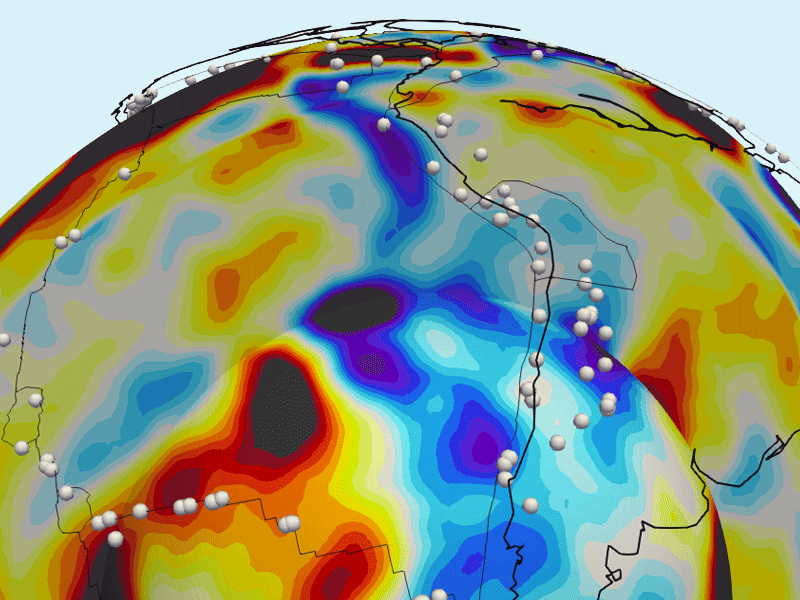
\includegraphics[width=0.5\textwidth]{geophysics_image_11-19-2023.png}
            \label{fig:motivation}
        \end{figure}
        \pause 
        \begin{itemize}
            \item Oil
            \item Ore deposits
            \item Water reservoirs
        \end{itemize}
    \end{itemize}
\end{frame}
\section{The Dirchlet-to-Neumann Map}
\begin{frame}{Dirichlet Problem}
    \begin{block}{Dirichlet Problem}
        A \textit{Dirichlet Problem} for a particular partial differential equation (PDE) is finding a function which solves the PDE on the interior of $\Omega$ given one that solves it on the boundary $\partial \Omega$ . 
    \end{block}
\end{frame}
\begin{frame}{Conductivity Problem}
    \begin{itemize}
        \item Conductivity function $\gamma(x)$
        \pause
        \item Voltage Potential function $f(x)$ on $\partial\Omega$
        \pause
        \item $u$ solves the Dirichlet problem for the conductivity equation: \[\begin{cases}
            \nabla\cdot(\gamma\nabla u)=0 & \text{ in }\Omega \\ u=f&\text{ on }\partial\Omega
        \end{cases}.\]
    \end{itemize}
\end{frame}
\begin{frame}{Dirichlet-to-Neumann Map}
    \begin{block}{Dirichlet-to-Neumann map}
        \[\Lambda_{\gamma}f=\gamma\frac{\partial u}{\partial \nu}\bigg|_{\partial \Omega}\]
    \end{block}
    \pause \begin{itemize}
        \item Describes the current flowing through the boundary of $\Omega$. 
    \end{itemize}
\end{frame}
\begin{frame}{The Main Result}
    \begin{block}{Theorem}
        \begin{center}
            If $\Lambda_{\gamma_1}=\Lambda_{\gamma_2}$ on $\partial \Omega$, then $\gamma_1=\gamma_2$ on $\Omega$. 
        \end{center}
    \end{block}
    \begin{itemize}
        \item Recall that $\Lambda_{\gamma}$ is the Dirichlet-to-Neumann map for the positive conductivity function $\gamma$. 
        \item If two conductivity functions have the same Dirichlet-to-Neumann map on $\partial\Omega$, then they must be the same. 
    \end{itemize}
\end{frame}
\section{Complex Geometrical Optics Solutions}
\begin{frame}{CGOs}
    \begin{block}{Complex Geometrical Optics solutions}
      A Complex Geometrical Optics (CGO) solution to a PDE is of the form \[u(x)=e^{i\zeta\cdot x}(1+r(x))\]  
    \end{block}
\end{frame}
\begin{frame}{The Schrödinger Equation}
    \begin{block}{CGOs of the Schrödinger Equation}
        For a voltage potential $q\in L^{\infty}(\Omega),$ the Schrödinger equation \[(\Delta+q)u=0\text{ in }\Omega\] has a complex geometrical optics solution of the form \[u(x)=e^{\zeta\cdot x}\gamma^{-\frac{1}{2}}(x)\left(1+O\left(\frac{1}{|\zeta|}\right)\right), \ |\zeta|\to\infty.\]
    \end{block}
    \pause
    \begin{itemize}
        \item This CGO solution is the key to proving the uniqueness result. 
        %The intuition comes from the fact that the term with $\zeta$ vanishes as it goes to infinity, leaving us with an oscillatory function with very nice behavior, which is easy to work with. 
    \end{itemize}
\end{frame}
\section{Applications}
\begin{frame}{Detection of Corrosion}
    \begin{columns}
	\begin{column}{0.5\textwidth}
   		\begin{figure}
   		    \centering
   		    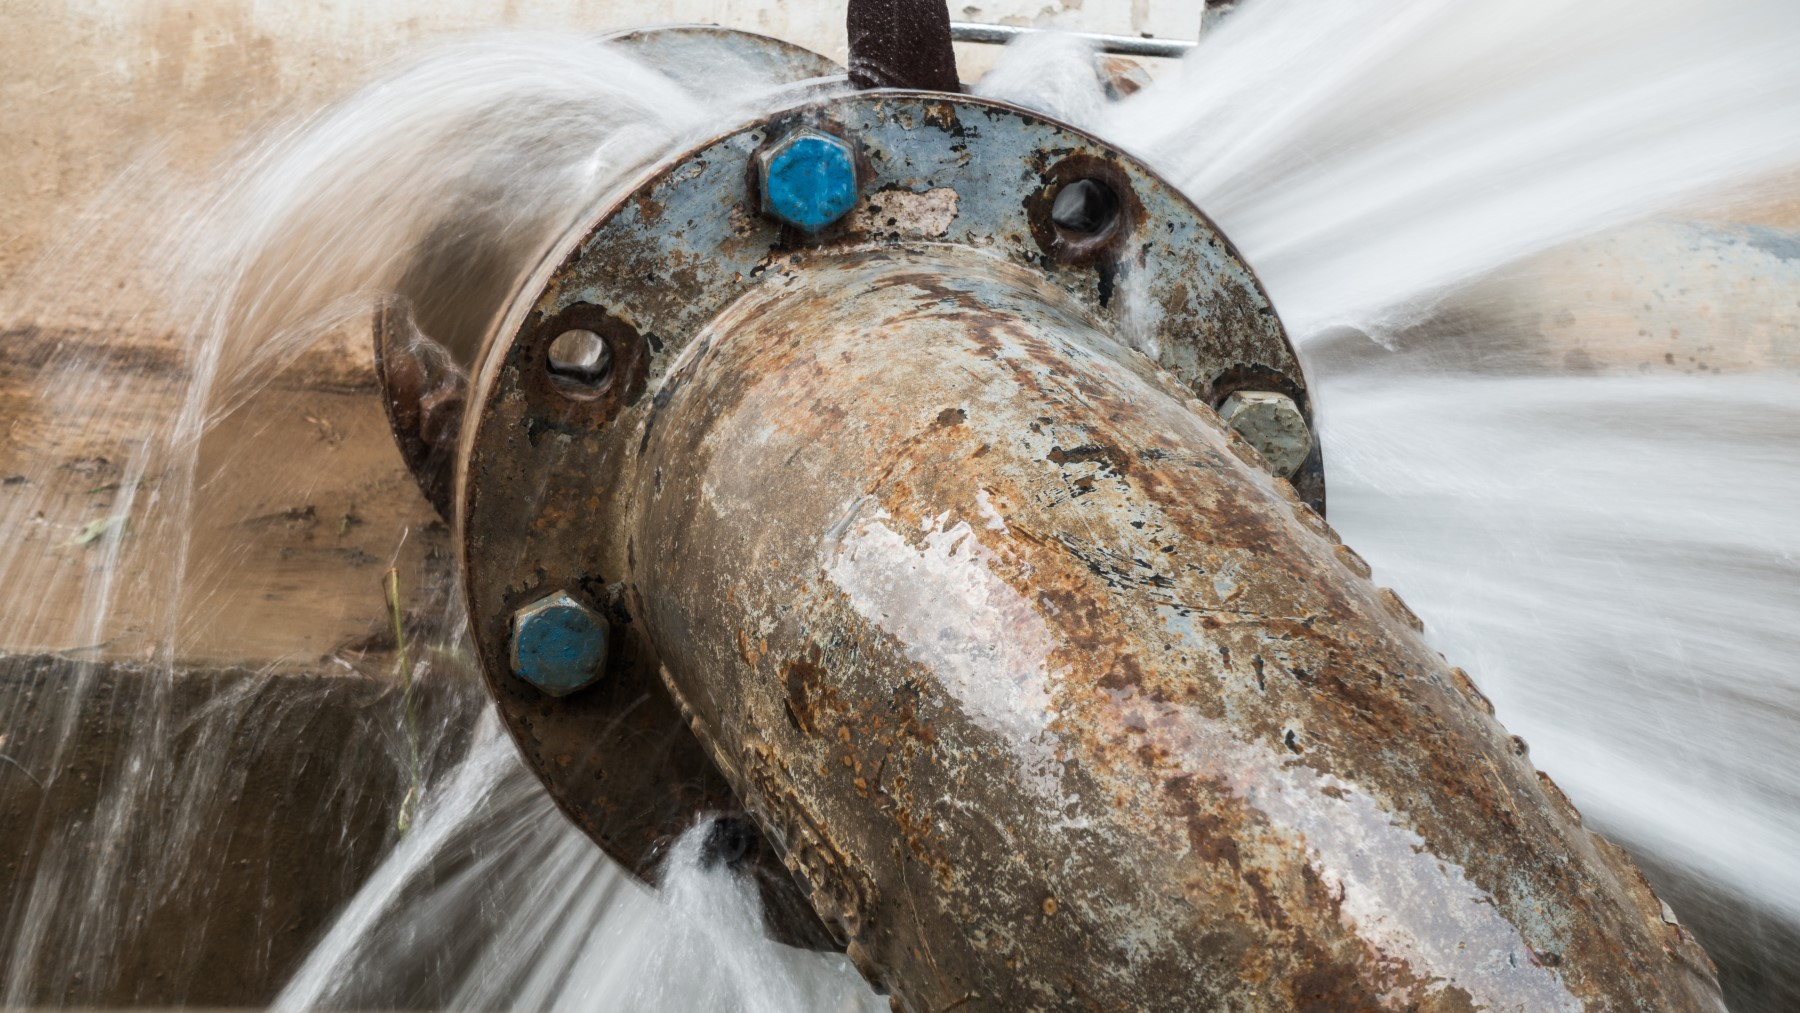
\includegraphics[width=0.8\textwidth]{pipebursting_photo_11-19-2023.jpeg}
   		    \label{fig:pipe}
   		\end{figure}
	\end{column}
	\begin{column}{0.5\textwidth}
   		\begin{itemize}
   		    \item Detection of cracks, corrosion, and leaks
         \item Nondestructive testing of materials
         
   		\end{itemize}
	\end{column}
 \end{columns}
\end{frame}
\begin{frame}{Electrical Impedance Tomography}
    \begin{columns}
	\begin{column}{0.5\textwidth}
   		\begin{figure}
   		    \centering
   		    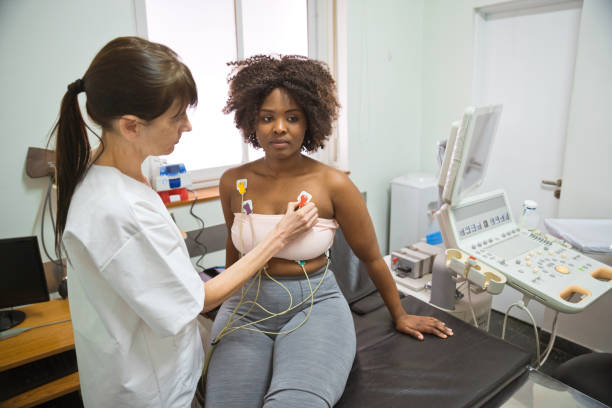
\includegraphics{ecg_photo_11-19-2023.jpeg}
   		    \label{fig:breast cancer}
   		\end{figure}
	\end{column}
	\begin{column}{0.5\textwidth}
   		\begin{itemize}
   		    \item Early Detection of Breast Cancer
         \item Monitoring Lung Health
   		\end{itemize}
	\end{column}
    \end{columns}
\end{frame}
\appendix
\section{Thank You!}
{\BackgroundShaded
\begin{frame}{\hspace{4cm} Thank you!}
% BLANK FRAME AT THE END, can add a thank you!
\end{frame}
}
%===============================================================%
\end{document}
%===============================================================% 